\documentclass{article}

% if you need to pass options to natbib, use, e.g.:
% \PassOptionsToPackage{numbers, compress}{natbib}
% before loading nips_2018

% ready for submission
\usepackage{nips_2018}

% to compile a preprint version, e.g., for submission to arXiv, add
% add the [preprint] option:
% \usepackage[preprint]{nips_2018}

% to compile a camera-ready version, add the [final] option, e.g.:
% \usepackage[final]{nips_2018}

% to avoid loading the natbib package, add option nonatbib:
% \usepackage[nonatbib]{nips_2018}

\usepackage[utf8]{inputenc} % allow utf-8 input
\usepackage[T1]{fontenc}    % use 8-bit T1 fonts
\usepackage{hyperref}       % hyperlinks
\usepackage{url}            % simple URL typesetting
\usepackage{booktabs}       % professional-quality tables
\usepackage{amsfonts}       % blackboard math symbols
\usepackage{amsmath}
\usepackage{nicefrac}       % compact symbols for 1/2, etc.
\usepackage{microtype}      % microtypography
\usepackage{graphicx}
\usepackage{subcaption}

\title{arXiv vs. snarXiv}

\renewcommand{\P}{\mathbb{P}}
\newcommand{\V}{\mathcal{V}}
\newcommand{\R}{\mathbb{R}}
\newcommand{\Z}{\mathbb{Z}}


% The \author macro works with any number of authors. There are two
% commands used to separate the names and addresses of multiple
% authors: \And and \AND.
%
% Using \And between authors leaves it to LaTeX to determine where to
% break the lines. Using \AND forces a line break at that point. So,
% if LaTeX puts 3 of 4 authors names on the first line, and the last
% on the second line, try using \AND instead of \And before the third
% author name.

\author{Tyler Blanton \And Sam Kowash}
  %% examples of more authors
  %% \And
  %% Coauthor \\
  %% Affiliation \\
  %% Address \\
  %% \texttt{email} \\
  %% \AND
  %% Coauthor \\
  %% Affiliation \\
  %% Address \\
  %% \texttt{email} \\
  %% \And
  %% Coauthor \\
  %% Affiliation \\
  %% Address \\
  %% \texttt{email} \\
  %% \And
  %% Coauthor \\
  %% Affiliation \\
  %% Address \\
  %% \texttt{email} \\


\begin{document}
% \nipsfinalcopy is no longer used

\maketitle

\begin{abstract}
We attempt to construct classifiers that can accurately distinguish between real arXiv \texttt{hep-th} abstracts and fake abstracts generated from a context-free grammar by the program snarXiv\footnote{\url{http://davidsd.org/2010/03/the-snarxiv/}}.
We study the bag-of-words and $n$-grams language models as well as several different classifiers: naive Bayes, likelihood-ratio, and tf-idf.
We find the likelihood-ratio and tf-idf methods to perform extremely well, classifying abstracts correctly with nearly 100\% accuracy.
\end{abstract}




\section{Introduction} \label{sec:intro}
The arXiv is a free online repository maintained by Cornell for preprints of scientific papers (many of which go on to be published in journals) from fields including mathematics, physics, and computer science.
Submissions are moderated via an endorsement system to ensure that only legitimate papers are posted, making it a valuable resource for scientists in many disciplines. In many areas of theoretical physics, almost all new papers are posted to the arXiv before publication.

The snarXiv is a computer program created by physicist David Simmons-Duffin that generates titles and abstracts in the style of arXiv's high-energy theory section (\texttt{hep-th}) using a context-free grammar.
Simmons-Duffin created a browser game, ``arXiv vs. snarXiv,''\footnote{Now sadly defunct, it appears, but some results are summarized at \url{http://davidsd.org/2010/09/the-arxiv-according-to-arxiv-vs-snarxiv/}} in which readers are presented with two title/abstract pairs---one from \texttt{hep-th}, the other generated with snarXiv --- and are asked to choose which one is real.
After 750,000 guesses, the success rate was only 59\%; i.e., people mistakenly identified a randomly-generated snarXiv title/abstract as real 41\% of the time.
This turns out to be a task that humans are remarkably (and amusingly) bad at, so we here investigate whether machines are any better.

In the first part of this report, we discuss the principles of our text representation (\S\ref{sec:LMs}) and classification (\S\ref{sec:classifiers}) schemes.
In the second, we present the results of parameter tuning and final classification accuracies. Details of implementation are collected in Appendix~\ref{app:details}.












\section{Theory}
Each of the abstract classification algorithms we use consists of three main parts: a parser, a language model, and a classifier.
Here we discuss the theory behind our language models and classifiers; details about our parsing choices can be found in Appendix~\ref{app:parsing}.
 
\subsection{Language models} \label{sec:LMs}
\subsubsection{\texorpdfstring{$n$-grams}{n-grams}} \label{sec:n-grams}
Assume that each abstract $X$ has a probability $\P(X|Y)$ of being from source $Y\in\{-1,1\}$, where $Y=1$ represents the label ``snarXiv'' and  $Y=-1$ represents the label ``arXiv.''
Suppose $X=(w_1,w_2,\ldots,w_N)$ is an abstract containing $N$ words $\{w_i\}_{i=1}^N$, and let $w_i^{i+k}$ denote the word sequence $(w_i,w_{i+1},\ldots, w_{i+k})$.
The $n$-grams language model approximates $\P(X|Y)$ as
\begin{align}
  \P(X|Y) = \P(w_1^N|Y) &= \prod_{i=1}^N \P(w_i|w_1^{i-1},Y)
  \\
  &\approx \prod_{i=1}^N \P(w_i| w_{i-n+1}^{i-1},Y) \quad\; (n\text{-grams approx.})
\end{align}
In other words, in the $n$-grams model we assume that the probability of a given word $w$ occurring in some abstract only depends on what the previous $n-1$ words in the abstract are, where $n$ is some (typically small) positive integer; the $n-1$ words on which $w$ depends are called the ``context'' of $w$.

In the simplest case $n=1$, each word occurrence is assumed to be completely independent of any context, which is why the 1-gram language model is often referred to as the ``bag-of-words'' (BoW) model.
Given some training set of abstracts from source $Y$, we define our BoW training estimate $\widehat\P(X|Y)_\text{BoW}$ as
\begin{align}
  \widehat\P(X|Y)_\text{BoW} &=  \widehat\P(w_1^N|Y)_\text{BoW} \equiv \prod_{i=1}^N \widehat\P(w_i|Y), \\
  \text{where } \quad \widehat\P(w_i|Y) &\equiv \frac{C_Y(w_i)+1}{\sum_w [C_Y(w)+1]} = \frac{C_Y(w_i)+1}{\sum_{w\in\V} C_Y(w)+V},
\end{align}
$C_Y(w_i)$ is the number of times that $w_i$ appears, $\V$ is a vocabulary of size $V=|\V|$ containing all of the words that we wish to learn about, and $\sum_{w\in\V} C_Y(w)$ is the total number of words in the training set.
The extra $+1$ on each word count $C_Y(w)$ comes from Laplace smoothing, which is a precautionary measure taken to prevent zero probabilities from occurring in cases where we need to classify an abstract that contains a word that did not appear in the training set.
Other technical details regarding bag-of-words and $n$-grams implementation (including parsing) can be found in Appendix~\ref{app:details}. 

The generalization to $n>1$ is straightforward: we define our estimate $\widehat\P(X|Y)_{n\text{-gram}}$ for a given training set from source $Y$ to be
\begin{align}
  \widehat\P(X|Y)_{n\text{-gram}} = \widehat\P(w_1^N|Y)_{n\text{-gram}} &\equiv \prod_{i=1}^N \widehat\P(w_i| w_{i-n+1}^{i-1},Y),
  \\
  \text{where } \quad \widehat\P(w_i|w_{i-n+1}^{i-1},Y) &\equiv \frac{C_Y(w_{i-n+1}^i)+1}{C_Y(w_{i-n+1}^{i-1})+V},
\end{align}
$C_Y(w_{i-n+1}^i)$ is the number of times that the $n$-gram $w_{i-n+1}^i$ occurs, and $C_Y(w_{i-n+1}^{i-1})$ is the number of times that the $(n-1)$-gram $w_{i-n+1}^{i-1}$ appears.

Note that since a typical arXiv/snarXiv abstract contains roughly 100 words, so the abstract probability $\P(X|Y)=\prod_{i=1}^N \P(w_i|w_1^{i-1},Y)$ is a product of $N\approx100$ different word probabilities, each of which is typically much less than one.
As a result, the size of $\P(X|Y)$ is heavily dependent on the abstract length and is usually extremely small, causing our estimates to hit numerical underflow in some cases.
To combat the issue of length dependence, we prefer to work with the perplexity
\begin{align}
  \text{PP}(X|Y) \equiv \sqrt[N]{\frac{1}{\P(X|Y)}} = \left[ \prod_{i=1}^N \P(w_i|w_1^{i-1},Y) \right]^{-1/N},
\end{align}
which normalizes the abstract probability by taking the geometric mean of the individual word probabilities (and inverting).
To prevent numerical underflow from rendering our algorithms useless, we always work with logs of probabilities in our code, which turns products into sums and keeps the numbers reasonable.
Note that the log of the perplexity is a simple arithmetic mean:
\begin{align}
  \log\text{PP}(X|Y) = -\frac{1}{N}\log\P(X|Y) = -\frac{1}{N} \sum_{i=1}^N \log\P(w_i|w_1^{i-1},Y).
\end{align}
In practice, we use the logs of the classification conditions given below in Section~\ref{sec:classifiers} to classify our test abstracts as arXiv or snarXiv; we only exponentiate back to perplexities for the purposes of figures.




\subsubsection{tf--idf}
The family of $n$-gram models can be used to produce term probabilities for naive Bayes or likelihood-ratio testing, but they also induce perfectly good $\tfrac{V!}{(V-n)!}$-dimensional vector representations of documents, where each entry records the occurrence of a given $n$-gram in the document.
These vectors are large, but fairly sparse, and make rudimentary features for regression or clustering algorithms. We enhance this model using the term-frequency--inverse-document-frequency (tf--idf) scheme as described in \citet[ch. 6]{jurafsky2014speech}.


% However, the \emph{semantic} model implied by raw count vectors is extremely crude. For example, ubiquitous words like ``the'', ``and'', and ``of'' are assigned great weight, and pull most document vectors in a handful of directions, distorting the representation space in a way that can make clusters harder to separate.
% This motivates a weighting scheme that recognizes words more unique to particular documents or classes; in particular, we developed feature vectors using the term-frequency--inverse-document-frequency (tf--idf) scheme as described in \citet[ch. 6]{jurafsky2014speech}.

Each entry $d_i$ in a document vector $d$ corresponds to a term $w_i$ in the vocabulary and receives a weight
%
\begin{align}
  d_i &= \mathrm{tf}_{i,d} \cdot \mathrm{idf}_{i}.
\end{align}
%
We define
%
\begin{align}
  \mathrm{tf}_{i,d} &\equiv \begin{cases}
                         1 + \log_{10}C_{i,d} &:\quad C_{i,d} > 0\\
                         0 &:\quad\text{else}
                       \end{cases},
\end{align}
%
where $C_{i,d}$ is the number of occurrences of $w_i$ in the document $d$, and
%
\begin{align}
  \mathrm{idf}_i &\equiv \log_{10} \frac{N+1}{\mathrm{df}_i + 1},
\end{align}
%
where $N$ is the number of documents in the training corpus, and $\mathrm{df}_i$ is the number of documents containing $w_i$.
%
\footnote{Our definition of $\mathrm{idf}_i$ varies from that given in the reference by smoothing terms which deal with the possibility of developing features from a corpus smaller than the one that produced the vocabulary and prevent infinite logs.}

The principle of tf--idf is to weight vector components according to their discriminating power: our representation should emphasize the most unique parts of documents.
Accordingly, the inverse document frequency metric completely ignores a word that occurs in every document, but gives great weight to a word occurring only once in the corpus.
Further, our term-frequency metric grows sublinearly, since a word occurring ten times is not necessarily ten times as important as one occurring singly.











\section{Classifiers} \label{sec:classifiers}
\subsection{Naive Bayes classifier}
Our first attempt at creating a program that distinguishes between arXiv and snarXiv abstracts utilized a naive Bayes (NB) classifier.
The theory behind this classifier is simple: if $\P(Y=1|X) > \P(Y=-1|X)$, then we classify $X$ as snarXiv; otherwise, we classify it as arXiv.
We can use Bayes' theorem $\P(Y|X) = \frac{\P(Y)\P(X|Y)}{\P(X)}$ to rewrite this classification condition as
\begin{align}
  \widehat{Y}_{NB} \equiv \arg\max_{Y\in\{-1,1\}} \P(Y)\P(X|Y). \label{eq:Bayes}
\end{align}
We estimate each probability in \eqref{eq:Bayes} by training on a large number of arXiv and snarXiv abstracts.
We define our estimate%
\footnote{The probabilities $\P(Y=\pm1)$ are somewhat trivial since we generate the snarXiv abstracts ourselves and can control over how many arXiv vs. snarXiv abstracts will be in the train and test sets. Since the snarXiv was originally created to make abstracts that compete one-on-one with arXiv abstracts, we chose to set $\P(Y=\pm1)=\tfrac{1}{2}$ for all tests reported in this paper.}
%
for $\P(Y)$ as the number of abstracts in training set $Y$ over the total number of abstracts in both the arXiv and snarXiv training sets.
The conditional probabilities $\P(X|Y)$ are more complicated, and are approximated using a language model from Section~\ref{sec:LMs}.



\subsection{Likelihood-ratio test}
A slightly more sophisticated classification rule is the likelihood-ratio (LR) test.
For a given abstract $X$, define the likelihood ratio $\Lambda(X)\equiv\frac{\P(X|Y=1)}{\P(X|Y=-1)}$.
While we certainly want our classifier to correctly label all snarXiv abstracts as fakes, we also want to minimize the probability that an arXiv abstract gets incorrectly classified as fake.
The Neyman-Pearson lemma states that the optimal classifier
\begin{align}
  \delta_{LR}^* \equiv \arg\max_\delta \P(\delta(X)=1|Y=1), \text{\; subject to \;} \P(\delta(X)=1|Y=-1)\leq \alpha
\end{align}
for any fixed false-positive tolerance $\alpha$ takes the form
\begin{align}
  \P\left(\delta_{LR}^*(X)=1\right) =
  \begin{cases}
    1,  & \Lambda(X) > \eta \\
    \gamma, & \Lambda(X) = \eta \\
    0,  & \Lambda(X) < \eta,
  \end{cases}
\end{align}
where $\eta$ and $\gamma$ can be treated as hyperparameters to be tuned in cross-validation.
In practice, $\gamma$ is almost completely irrelevant since for any $\eta$, the odds that a language model like $n$-grams would yield an estimate for $\Lambda(X)$ that is \textit{exactly} equal to $\eta$ are essentially zero.%
\footnote{The borderline case of the naive Bayes classifier where $\P(Y=\pm1|X)=\frac{1}{2}$ is irrelevant for the same reason.}
%
We arbitrarily use $\gamma=0.5$, meaning the only hyperparameter we tune is $\eta$.
Because of the issues of small $\P(X|Y)$ probabilities discussed in Section~\ref{sec:n-grams}, it is more practical to instead compare the perplexities $\text{PP}(X|Y)=\P(X|Y)^{-1/|X|}$.
The relevant parameter in the LR-test is thus $\eta^{1/|X|}$. We would like our hyperparameter to not depend on the specifics of the input though, so we note that the average abstract length is about 120 words and define $\eta_\text{PP}\equiv \eta^{1/120}$ to be our new LR-hyperparameter.





\subsubsection{Logistic regression}
For weighted vector representations as produced by the tf--idf scheme, it is not obvious how to produce term or document likelihoods for use in a Bayes or LR classifier, so we must turn to other classification methods. Fortunately, there are a host of methods for binary classification of vector data, and it is convenient and familiar to choose regularized logistic regression. We adopt a model
%
\begin{align}
  \P(Y=y \mid x) &= \frac{1}{1 + e^{-y w^T x}}
\end{align}
%
where $y \in \{-1, 1\}$ represents the class of a document (negative for arXiv, positive for snarXiv), $x$ is a tf--idf document vector, and $w$ and $b$ are parameters to be learned. We accomplish this by minimizing the convex regularized objective
%
\begin{align}
  J(w) &= \sum_{i=1}^N \log\left[1+ \exp\left(-y_i(x_i^T w + b)\right)\right] + \lambda \|w\|_2^2,
\end{align}
%
where $\lambda$ is a hyperparameter. The optimum lacks a closed form, but it can be found easily in CVXPY even for the $V \sim 15000$-dimensional space created by our vocabulary. After training $w$ and $b$, we classify a document according to the sign of the exponent $(x_i^T w + b)$, since it can be related to the log-ratio of probabilities to be in each class.







\section{Results}
We report results for three different algorithms: bag-of-words model with naive Bayes classifer (BoW-NB), bag-of-words model with likelihood-ratio test (BoW-LR), and bigrams=(2-grams) model with likelihood-ratio test (bi-LR).
In each case, we trained on an equal number $N_\text{train}^Y=1000$ of arXiv and snarXiv abstracts, and we also tested on 1000 arXiv abstracts and 1000 snarXiv abstracts.
%
% Add tf-idf stuff?
%

For BoW-NB, we found the classification accuracy to be 77\%, with the only misclassifications being false positives (arXiv abstracts that the classifier mistakes as snarXiv); when a snarXiv abstract is tested, it is correctly identified as snarXiv 100\% of the time.
This is somewhat expected for a classifier which does nothing to constrain the false-positive rate.

For BoW-LR and bi-LR, we tuned the LR-hyperparameter $\eta_\text{PP}$ through cross-validation to maximize the classification accuracy on abstracts from both arXiv and snarXiv.
We found $\eta_{\text{PP}}=0.7$ to perform best in both models; Figure~\ref{fig:histograms} shows histograms of our estimates for $\frac{\text{PP}(X|\text{snarXiv})}{\text{PP}(X|\text{arXiv})}$ for both the arXiv and snarXiv test corpora.
The LR-classifier is clearly distinguishing between the two sets, giving a classification accuracy of 100\%.








%\begin{figure}[!htbp]
%\centering
% \includegraphics[width=0.48\textwidth]{../figures/FDR_TPR_plot_BOW.png}
%%\caption{LR-classifier using bag-of-words model.}
%\end{figure}

\begin{figure}[!htbp] 
\centering
\begin{subfigure}[t]{0.48\textwidth}
  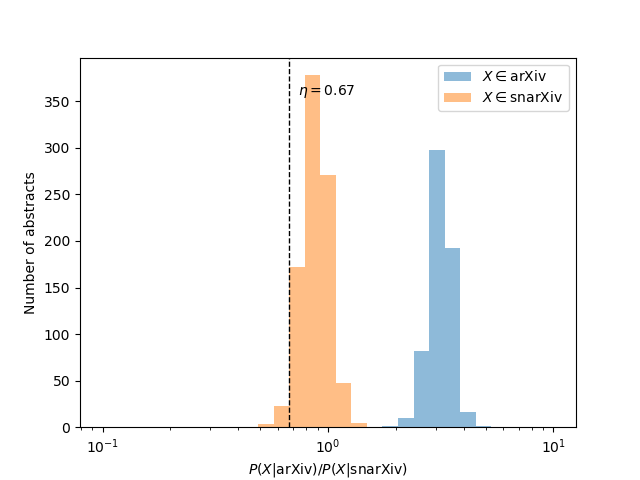
\includegraphics[width=\textwidth]{../figures/BOW_histogram.png}
  \caption{BoW-LR model}
\end{subfigure}
  \hfill
\begin{subfigure}[t]{0.48\textwidth}
  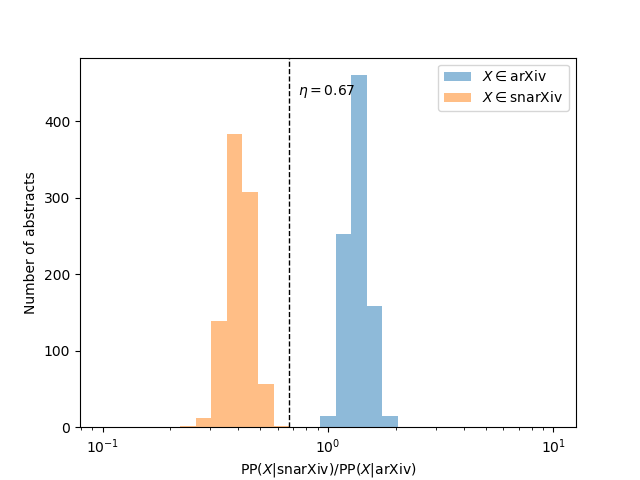
\includegraphics[width=\textwidth]{../figures/bigram_histogram.png}
  \caption{bi-LR model}
\end{subfigure}
\caption{Perplexity ratio histograms for both LR-models. The dotted black line corresponds to $\eta_\text{PP}=0.7$.}
\label{fig:histograms}
\end{figure}

Logistic regression trained on 2000 tf--idf document vectors and tested on 8000 yielded error rates ranging from 0.05\% to 0.375\% depending on the regularization parameter (lower $\lambda$ tended to produce lower error, even down to $\lambda \sim 10^{-8}$), and exhibited the same pattern as the Bayes and LR classifiers of 100\% accuracy at identifying snarXiv papers. The only errors at any regularization scale were misidentification of arXiv papers.








\section{Conclusion}
We have demonstrated that the arXiv--snarXiv discrimination problem, while unusually difficult for humans, yields to even very simple analytical frameworks. This is most likely due to the profound different statistical structures of the corpora illustrated in our histograms, which are not evident to human inspection (which focuses on attempting to parse or impart semantic structure) but stand out readily to probabilistic classification methods.















% \subsection{Possible extension}
% Our results thus far suggest that the language produced by snarXiv may just be too artificial and constrained to put up much of a fight in the classification task.
% The naive Bayes classifier never mistakes a snarXiv paper for real, although it still accidentally flags a decent chunk of real papers as fake.
% We will continue this work with more sophisticated feature generation and classifiers to explore different methods and try to reduce the remaining error, but it is worth looking in other directions as well.

% In particular, if snarXiv cannot produce abstracts that are convincing to our classifier, what can?
% The field of generative adversarial networks has become prominent recently, as reviewed in \citet{creswell2018generative}, and we are considering extending our project in this direction.
% The aim would be to produce, effectively, a next-generation snarXiv that achieves a meaningful error rate against its discriminating counterpart.
% Several sources note that GANs are not naturally suited to contexts with discrete data streams, so this may prove unworkable, but is one direction to pursue if our original plan leads to shallow results.





\appendix
\section{Technical details} \label{app:details}
\subsection{Parsing abstract text} \label{app:parsing}
Our parser attempts to translate the raw abstract text (a string) to a list of formatted words that are easily identifiable between different abstracts.
We first split the text on all spaces, newlines, and hyphens, and for uniformity we make all words lowercase.
Next, we look for words that end in a period or question mark and insert the special word tokens \texttt{<e>} and \texttt{<s>} afterwards to mark the end of one sentence and the start of another.
Lastly, we strip out all punctuation (except for the special tokens), prepend \texttt{<s>} to the list (marking the start of the first sentence), and delete the last word if the list ends \texttt{<e>} \texttt{<s>} (otherwise, we append \texttt{<e>}).

An example of parser input/output is

Input: \texttt{``I'm taking a CSE class on machine-learning.\ It's a lot of work, but pretty interesting.''}

Output: \texttt{[<s>, im, taking, a, cse, class, on, machine, learning, <e>, <s>, its, a, lot, of, work, but, pretty, interesting, <e>]}, 

where each ``word'' in the output list is a string.

Our parsing scheme works well, but it leaves traces of some TeX commands from the raw abstract text; for example, it sends \texttt{\textbackslash mathbb\{Z\} $\to$ mathbbz}.
This would be fine if all arXiv and snarXiv abstracts have TeX commands written the same way, though it is possible in some cases for abstracts to write the same command in different ways. In practice, we find that these instances are rare enough for the concern to be negligible.


\subsection{Vocabulary}
We defined our vocabulary $\V$ as the collection of $V=15,315$ unique words that appeared at least twice in a training corpus of 12,000 randomly chosen parsed arXiv abstracts and 12,000 (randomly generated) parsed snarXiv abstracts.
We decided not to include the 13,960 words that only appeared once since they seem to be relatively uncommon (often they are the residuals of TeX commands), and including them would nearly double our vocabulary size.
This pruning can be thought of as a feature-processing step.


\subsection{\texorpdfstring{$n$-grams}{n-grams}}
It is fairly common for a word to appear in the test set that is not in the vocabulary.
When this happens, we change the word to a special token \texttt{<UNK>}.
We then treat \texttt{<UNK>} as we would any other word when counting $n$-gram occurrences $C_Y(\cdot)$.

We prepend copies of the start sentence token \texttt{<s>} to each parsed abstract to ensure that the first $n$-gram consists of $n-1$ copies of \texttt{<s>} and one ``real'' word.
Similarly, we append copies of \texttt{<e>} to the end of each parsed abstract.





\nocite{sahami1998bayesian,ngram-cat,textclass,trivedi2016study,cvxpy,cvxpy_rewriting}

\bibliographystyle{plainnat}
\bibliography{references}
\end{document}
